\documentclass[main.tex]{subfiles}
\usepackage{floatrow}
\usepackage{float}
\usepackage{bm}
\usepackage{amsmath}
\usepackage{amssymb}
\begin{document}

\section{Machine Learning Theory}
Throughout this section the theory of machine learning that will be used in this thesis is described and explained.

\subsection{Motivation}
It can be difficult for humans to recognize certain patterns and trends in data. This becomes more difficult the greater the quantity of the data is, which is becomming more and more common with the rapidly growing topic of \textit{Big Data}. For this reason, computers are often used instead of humans to recognize patterns and trends in the data by analyzing the data, which is what is called \textit{Machine Learning}. In this thesis, we will use machine learning in section \textbf{MANGLER REFERENCE} to develop a model to estimate the 2D pose of a single human in an image. Later, in section \textbf{MANGLER REFERENCE}, we will use machine learning to improve our understanding of the model.

\subsection{Machine Learning Paradigms}
Machine learning is usally split into the following three paradigms
\begin{enumerate}
    \item \textit{Supervised learning} where the data consists of features and labels. By analyizing the data the algorithm learns to predict the labels given the features \cite{ESL}. Supervised learning is further split into \textit{classification} and \textit{regression}. If the value of each label is limited, then the task is a classification task. If the value of each label is not limited, then the task is a regression task. 
    \item \textit{Unsupervised learning} where the data only consists of features. The algorithm then learns properties of the data, without any provided labels \cite{ESL}.
    \item \textit{Reinforcement learning} where the algorithm learns to perform the action in a given environment that yields the highest reward \cite{PRML}.
\end{enumerate}
In this thesis we will make use of supervised learning when developing our model for pose estimation. Later, unsupervised learning is used when we explore our developed model.

\subsection{Evaluation of Machine Learning Models}
When developing a machine learning model it is important to know how trustworthy the developed model is. This is usually done by testing how good the model is at generalizing unseen data, which is done by making use of \textit{evaluation metrics}.

\subsubsection{Splitting the dataset}
When developing a machine learning model, the data needs to both create the model, but also to evaluate the model. For the evaluation of the model, one of the two following techniques is usually used

\begin{enumerate}
    \item \textit{Cross validation} where the data is split into $K$ random non-overlapping chunks of equal size. The model is then trained for $K$ rounds on $K - 1$ of the chunks, where the last chunk is used for evaluating the model. After each round the parameters of the model is reset to ensure one round does not affect another round. After the $K$ rounds the average loss of the $K$ rounds is the loss of the model \cite{MAD_book}.
    \item \textit{Train-validation-test} where the data is split into $3$ random non-overlapping chunks. The training dataset is then used for training the model and the validation dataset is used for evaluating the model as it is being developed - this often means, that the \textit{hyperparameters}, the paramters that are not possible to fit from the data, are being tweaked to yield the best validation loss. Lastly, the testing dataset is used as a final evaluation of the model to yield an unbiased evaluation of the model. Once the testing dataset has been used it can no longer be used for evaluating the data, as this ensure an unbiased evaluation \cite{MAD_L3}.
\end{enumerate}
Throughout this thesis the train-validation-test technique will be used over cross validation for evaluating the developed models. This is done, since cross validation is better suited for smaller datasets, as the runtime is much greater than the runtime of the train-validation-test technique.

\subsubsection{Evaluation Metrics for Supervised Machine Learning (Loss Functions)}
When we have trained a model, we need to somehow evaluate how well the model performs on unseen data. This is usually done by making use of evaluation metrics or \textit{loss functions}. There are many different loss functions, each with their own advantages and disadvantages. One of the most common loss functions for regression is the \textit{Mean Squared Error (MSE)}, defined as
$$MSE = \frac{1}{n} \sum_{i = 1} ^n \left( y_i - \hat{y}_i \right)^2$$
where $y_i$ is the true value of the $i$th observation and $\hat{y}_i$ is the estimated value of the $i$th observation. Thus, $MSE$ measures the average squared difference between the true observation and the estimated observation. The aim of a model is thus to make the $MSE$ as small as possible \cite{ISL}.

\subsection{Neural Networks}
In recent years \textit{deep learning} and \textit{neural networks} have revolutionized the use of machine learning. In this thesis a neural network will be used for performing the human pose estimation.
\subsubsection{The Mathematics Behind Neural Networks}
\begin{figure}[H]
    \centering
    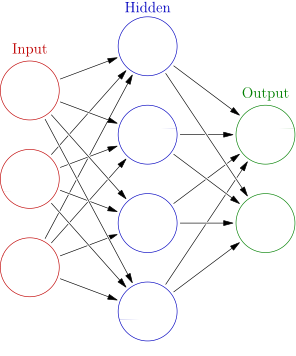
\includegraphics[height = 5 cm]{entities/feed_forward_nn.jpg}
    \caption{Visualization of a feedforward neural network with a single hidden layer \cite{feedforward_nn}}
    \label{feedforward_nn}
\end{figure}
\textbf{The architecture} \\
One of the most common types of neural networks are \textit{feedforward neural networks}, where the data flows unidirectionally through the network. Such a network is visualized in Figure \ref{feedforward_nn}. The network is built up of three types of components: the \textit{input layer}, the \textit{hidden layers} and the \textit{output layer}. Each layer is built up of \textit{units}, also called \textit{neurons} (which are visualized as circles in Figure \ref{feedforward_nn}), where each neuron has a \textit{bias} assigned to it, and is connected to one or two other layers through \textit{edges} (which are visualized as arrows in FIgure \ref{feedforward_nn}), where each edge has a \textit{weight} assigned to it. Hidden layers are connected to two other layers - one before the hidden layer and one after the hidden layer - where the input layer is only connected to the next layer in the network and the output layer is only connected to the previous layer in the network. \\
We can define the network mathemaically by letting $h_n ^{(i)}$ denote the value of the $n$th node in the $i$th layer, $w_{m, n}$ denote the value of the weight of the edge connecting the $n$th node in the $i$th layer to the $m$th node in layer $i + 1$ and $b_n ^{(i)}$ denote the bias corresponding to the $n$th node in the $i$th layer. \\
When data flows through the model it follows the following formula
$$\bm{h}^{(i + 1)} = g^{(i + 1)} \left( \bm{W}^{(i + 1)} \bm{h}^{(i)} + \bm{b}^{(i + 1)} \right)$$
where $\bm{W}^{(i + 1)}$ is the weights between layer $i$ and layer $i + 1$ defined by
\begin{center}
    \begin{math}
        \bm{W}^{(i + 1)} =
        \begin{pmatrix}
            w_{0, 0} & w_{0, 1} & \cdots & w_{0, n} \\
            w_{1, 0} & w_{1, 1} & \cdots & w_{1, n} \\
            \vdots & \vdots & \ddots & \vdots \\
            w_{m, 0} & w_{m, 1} & \cdots & w_{m, n}
        \end{pmatrix}
        ,
    \end{math}
\end{center}
$\bm{h}^{(i)}$ is the values of the nodes in the $i$th layer defined by
\begin{center}
    \begin{math}
        \bm{h}^{(i)} =
        \begin{pmatrix}
            h_{0} ^{(i)} \\
            h_{1} ^{(i)} \\
            \vdots \\
            h_{n} ^{(i)} \\
        \end{pmatrix}
        ,
    \end{math}
\end{center}
$\bm{b}^{(i + 1)}$ is the values of the biases of layer $i + 1$ defined by
\begin{center}
    \begin{math}
        \bm{b}^{(i + 1)} =
        \begin{pmatrix}
            b_{0} ^{(i + 1)} \\
            b_{1} ^{(i + 1)} \\
            \vdots \\
            b_{m} ^{(i + 1)} \\
        \end{pmatrix}
    \end{math}
\end{center}
and $g$ is an \textit{activation function}, that is typically applied element-wise \cite{DeepLearning} \cite{3b1b_1}. One often used activation function is the \textit{rectified linear activation function} (or \textit{ReLu} for short) defined by
$$g(x) = \max\{0, x\}.$$
The ReLu-function is very close to being linear, making the function keep many of the properties of linear functions that make them easy to optimize and generalizing, which are two great advantages of using the ReLu-function. Another great advantage of using the ReLu-function is stated by the \textit{universal approximation theorem} that states, that a feedforward network with a linear output layer and at least one hidden layer with the ReLu-function (or another activation function from a wide class of activation functions) can approximate any continuous function on a closed and bounded subset of $\mathbb{R}^n$, as long as the network has enough hidden neurons \cite{DeepLearning}. 
\noindent \textbf{Gradient Descent} \\
\noindent \textbf{Backpropagation} \\


\subsubsection{Termonology}
\textbf{Overfitting and Regularization} \\
% Lidt uenig med definitionen af overfitting - taget fra DeepLearning. Tænk på underfitting.
The main goal of a machine learning model is to generalize well on unseen data. This can often be difficult, as the model simply "remembers" the training data instead of learning the patterns in the training data. In other words, the gap between the training error and the test error is too large, which is a concept called \textit{overfitting}. Certain techniques are designed to reduce the test error - these techniques are collectively called \textit{regurlization} \cite{DeepLearning}. \\
\textbf{Mini-batch} \\
\textbf{Batch Normalization} \\
\textbf{Epoch} \\
\textbf{Optimizer} \\
\subsubsection{Convolutional Neural Networks}
\textbf{NN Upsampling} \\
\textbf{Maxpooling}
\subsubsection{Stacked Hourglass}
\textbf{Reasoning behind using the Stached Hourglass} \\
\textbf{The Residual Modules}\\
\textbf{The Hourglass}\\
\textbf{The Stacked Hourglass}

\subsection{Principal Components Analysis and K-means Clustering}
\subsubsection{Principal Components Analysis (PCA)}
\subsubsection{K-means Clustering}


\end{document}